\documentclass[a4paper, 12pt]{article}
\usepackage{graphicx}
\usepackage{listings}

\setlength\parindent{24pt}

\lstset{language=c++,breaklines=true, frame=single}

\begin{document}

\begin{figure}
    \centering
    
\includegraphics[width=1\textwidth]{Logo}
\end{figure}

\title{Assignment Part 2 Report}
\author{Manwel Bugeja}
\date{\today}
\maketitle

\tableofcontents
\newpage

\section{Question 1}
\subsection{How the problem was tackled} 
\subsubsection{Lexer}
For this part, "char" was added to the keyword\_type function within transitions.cpp. This was done so that "char" is identified as a keyword.
Apart from that, the square brackets where added to the transition tablle and classifier table. The states that the square brackets led to where added 
to the token\_type() function and to the list of accepting states. The updated part of the FSA is included as a figure.
\linebreak

As for the square brackets, these were simply added to the tables. The updated part of the FSA is included as a listing.

\begin{figure}[h]
    \centering
    \frame{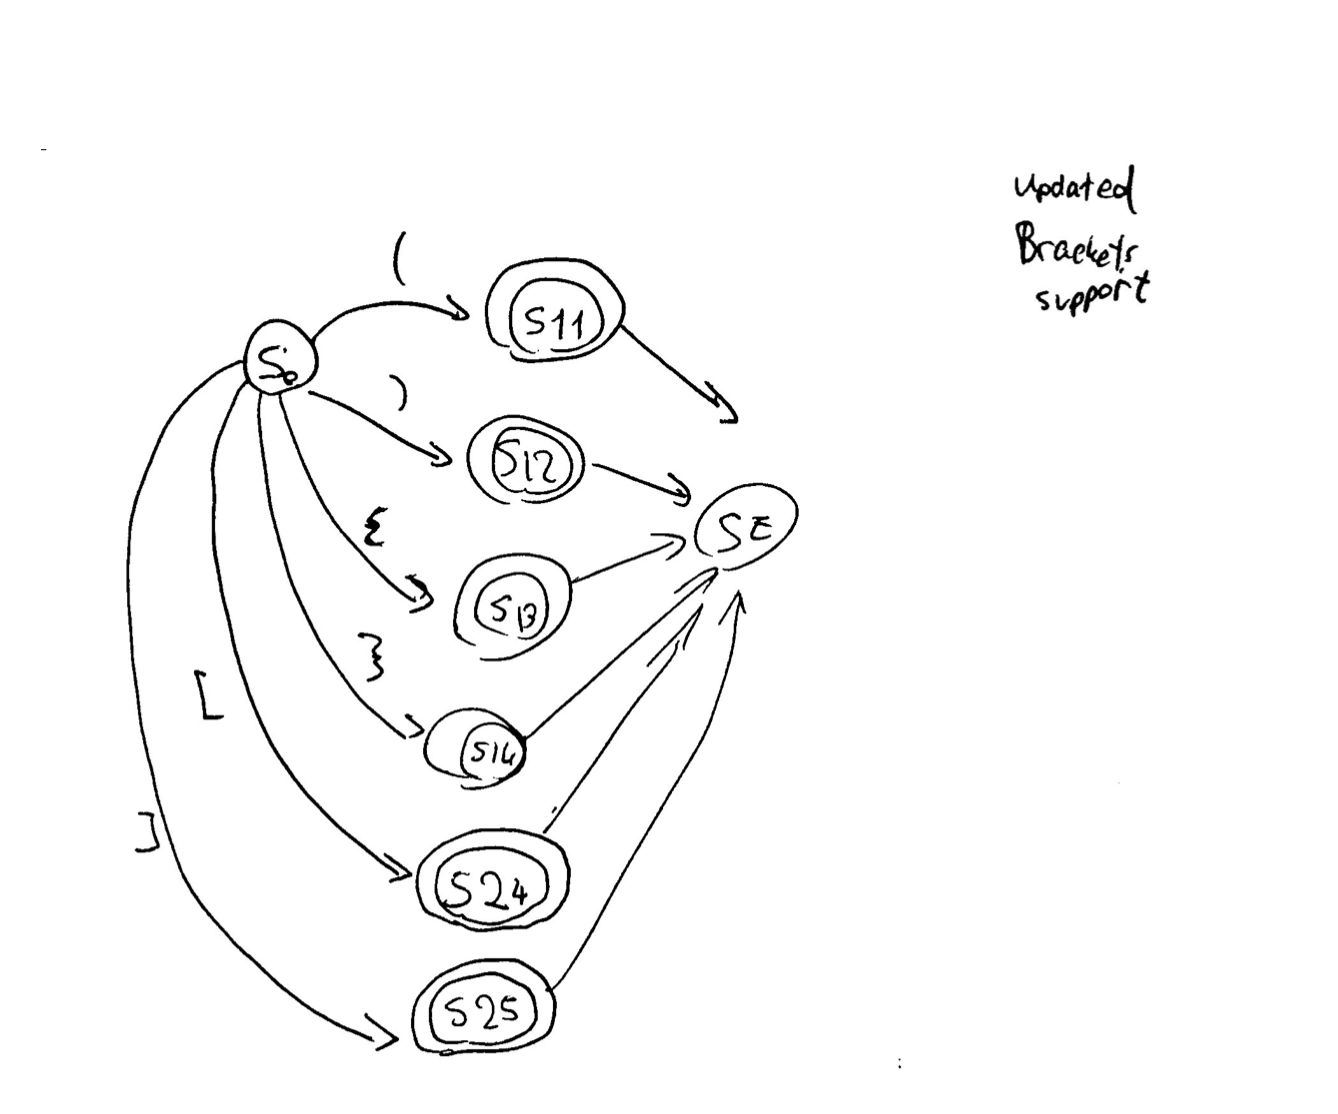
\includegraphics[width=1\textwidth]{images/brackets_updated}}
    \caption{FSA (part concerned with updated brackets)}
\end{figure}

\subsubsection{Parser}
From the parser side, char was added to the TYPE enum. This would enable the semantic anayser to declare chars when a char value is 
given after it. The array parsing line is included as a listing.

\begin{lstlisting}[caption=Array parsing]]
case identifier:    
    if (next\_token.type == scb) {
        //return parse_array();
    }
\end{lstlisting}

\section{Question 3}
For this task, the EBNF was changed into Antlr format. The script within the Antlr/ is run to generate the outputs
\end{document}
